\section{Investigating Trends}\label{sec:results}

SMA crossover-based partitioning of performance observations provides
a systematic method for grouping time-correlated performance events.
Once a divergence region (i.e., a performance trend) has been identified,
more focused statistical analyses can then be applied within the region
to gain insight into the factors that contributed to that trend.  Examples of
contributing factors may include utilization, system health, and component performance.
In the following analyses, we separate our 11,986 performance observations into sets of observations that all ran on the same test platform (as described in Table \ref{tab:platform-descriptions}) to characterize the factors that contribute to time-dependent performance variation across different file systems and architectures.

\subsection{Correlative analysis} \label{sec:results/correlate-mira}

\begin{figure}
    \centering
    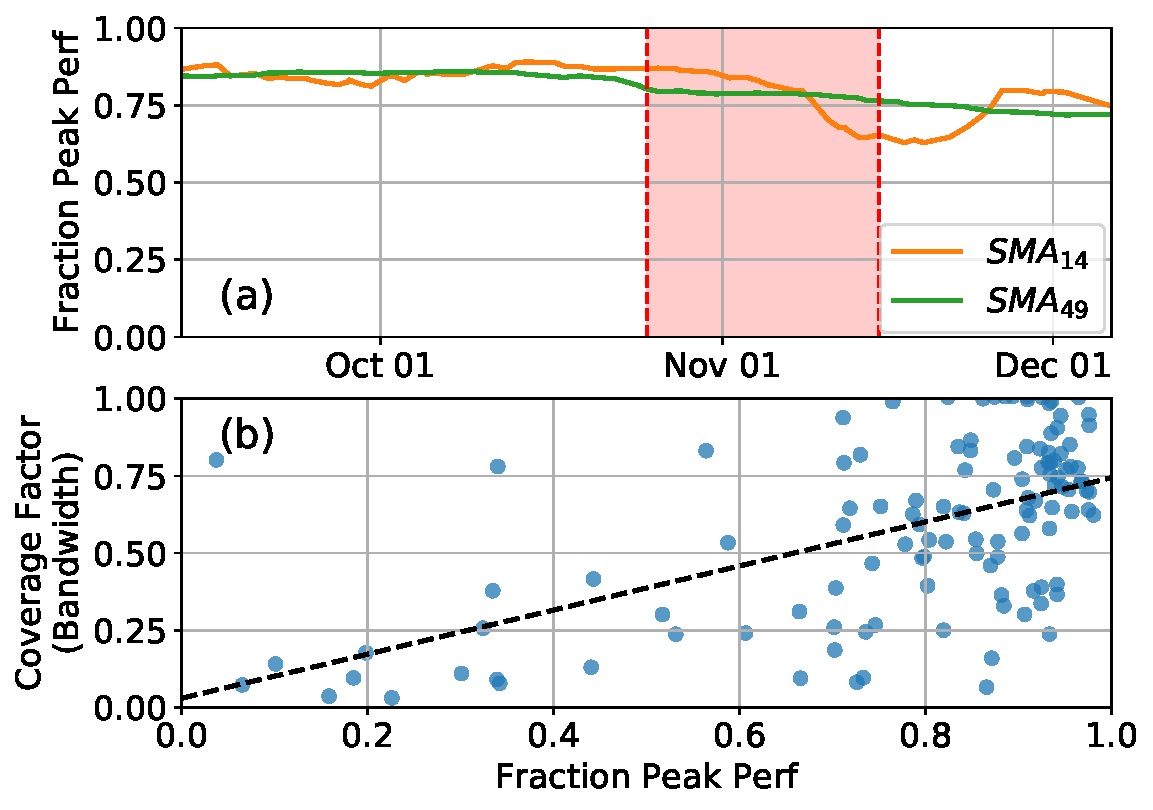
\includegraphics[width=1.0\columnwidth]{mira-correlation-region}
    \vspace{-.35in}
    \caption{Correlation between performance and $CF_{bw}$ in a divergence region on \mira for all I/O motifs combined.
    (a) highlights the divergence region of interest and corresponds to the same highlighted region shown in Fig. \ref{fig:mira-regions-overview}. (b) shows the correlation between performance and $CF_{bw}$ in that region.
    Correlation coefficient is $0.507$ and p-value is ${8.71 \times 10^{-9}}$; dashed line in (b) is a linear fit with slope $0.503$ drawn for visual aid.}
    \label{fig:mira-correlation-region}
    % source: sc18_region-correlation.ipynb
\end{figure}

% Bandwidth, IOPS, and metadata contention are confidently correlated with I/O performance at both long. 

\TODO{add a footnote explaining p-value}
We begin our correlative analysis by partitioning a year-long data set into
divergence regions using the method described in
Section~\ref{sec:features/partitioning}.  Using observations from \mira
\mirafsone as an example, we set ${w_{short} = \textup{two weeks}}$ and ${w_{long}
= \textup{seven weeks}}$ to identify divergence regions, and then discard any
regions with fewer than three data points.  Regions with few data points are discarded
for two reasons: (a) intuitively, very short divergence regions occur
when $\textup{SMA}_{short} \approx \textup{SMA}_{long}$ and there is
minimal long-term variation, and (b) statistically, it is impossible
to assert the statistical significance of a correlation with fewer than
three data points.  This yields 32 divergence regions.

We then apply Pearson correlation~\cite{Falk97manyfaces} to the feature vectors within each divergence region to identify the factors that correlate with its
performance trend.
The result of this process is a new feature vector for each divergence region which contains the correlation coefficients between the fraction of peak performance and every other attribute across all observations in that region.
We then use the p-value of each correlation coefficient\footnote{
The p-value of a correlation coefficient is the probability of observing data that would show the same correlation coefficient in the absence of any real relationship between the underlying metrics.
A low p-value indicates that it is extremely unlikely that the calculated correlation coefficient would be observed if the metrics being compared had no real correlation.
As such, p-values represent the statistical significance of a statistical measurement.}
to further downselect the total set of regions to those with extremely high significance
($\textup{p-value} < {1.0 \times 10^{-5}}$).
This threshold yields a total of nine relevant divergence regions on \mira \mirafsone which are all depicted as shaded extents in Figure \ref{fig:mira-regions-overview}.
Each of these nine regions exhibits at least moderate correlation ($R$) ranging from 0.507 to 0.884 with the bandwidth coverage factor feature.

\TODO{I'm not sure I understand why we're aggregating divergence regions from different motifs here, since everywhere else our analysis is applied to these independently. For one, different motifs could have different trend regions by definition. If the results hold over just one motif, maybe just use those, or something? -SS}
Fig.~\ref{fig:mira-correlation-region} illustrates the correlation between bandwidth coverage factor and fraction peak performance for a particular divergence region in November 2017 on \mira \mirafsone.
This example exhibits the lowest correlation ($R = 0.507$) with bandwidth coverage factor of any of the selected regions, and the scatter plot of performance results shows why:
this region contains a cluster of poorly performing probes (${0.2 < \textup{fraction peak perf} < 0.4}$) that ran with a relatively high bandwidth coverage factor.
This region is also the single largest divergence region observed on \mira; a difference of over 20\% between $\textup{SMA}_{short}$ and $\textup{SMA}_{long}$ was observed during this time.
This divergence region example highlights the importance of not just identifying regions and calculating correlations, but identifying cases in which the analysis indicates the presence of an unknown factor that is not adequately captured by the instrumentation framework.

Despite the unusual region shown in Fig. \ref{fig:mira-correlation-region},
however, these data indicate that the time-dependent performance divergences observed on \mira show either moderate or strong correlation with bandwidth contention.
Additionally, this correlation with performance degradation occurs across
\emph{all} I/O motifs (similar to Figure \ref{fig:regions-heatmap}a) which
distinguishes it from the motif-specific case discussed in Section
\ref{sec:features/timedependent}.  

When the same Pearson correlation is calculated across the entire collection
of \mira \mirafsone data in the absence of partitioning, the correlation with bandwidth coverage factor
yields an overall result of $R = 0.483$ and $\textup{p-value} =
2.25\times 10^{-88}$.  \textbf{Thus, significantly stronger
correlations can be found by focusing analysis on algorithmically identified regions of
interest in the data.}

% \TODO{We could use a plot for comparison if we have a lot of free time to
% kill.  I don't think it is critical though.}

\subsection{Survey of divergence regions} \label{sec:results/correlate-all}

% - Bandwidth, IOPS, and metadata contention are confidently correlated with I/O performance at both long. 



\begin{figure}
    \centering
    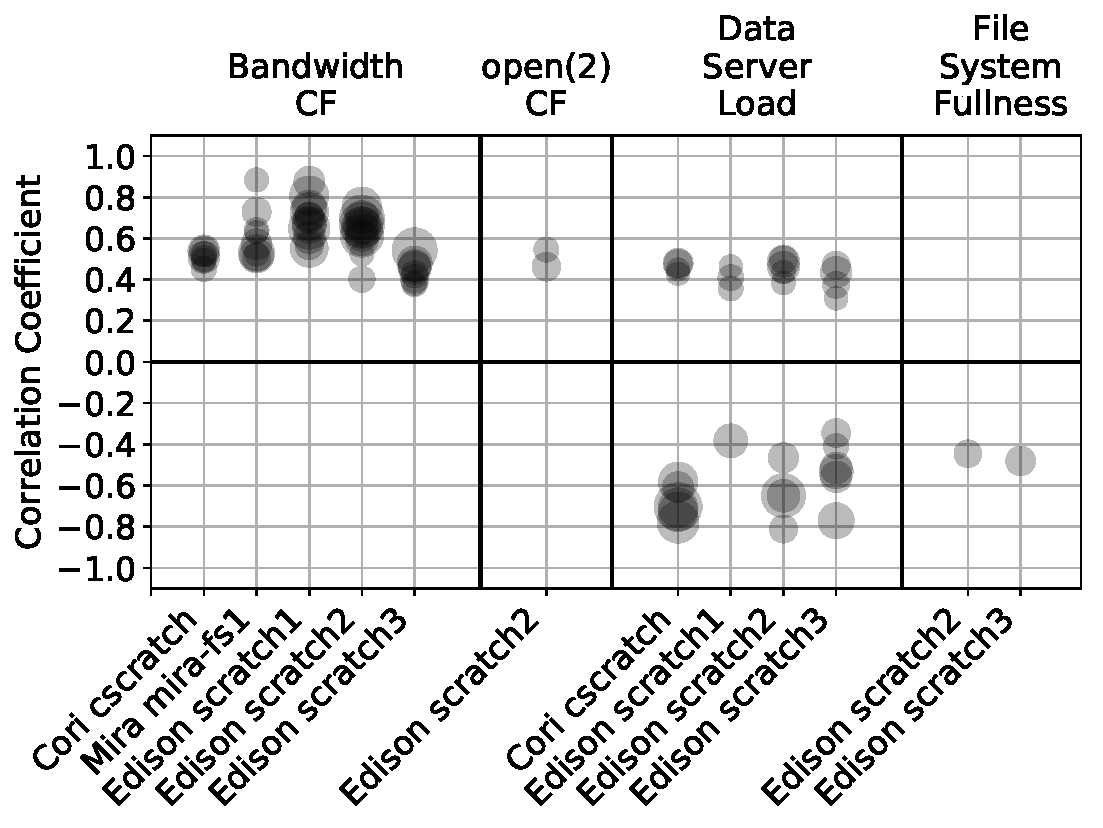
\includegraphics[width=1.0\columnwidth]{trend-correlations}
    \vspace{-.35in}
    \caption{Correlations discovered between fraction peak performance and all other attributes measured during job execution.
    Each circle represents the correlation coefficient over a single trend region, and its diameter is proportional to $-\log_{10}(\textup{p-value}$).
    CF denotes coverage factor.}
    \label{fig:trend-correlations}
    % source: sc18_region-correlation-all.ipynb
\end{figure}



Next we apply the same correlation analysis to the other test platforms in our study, again only keeping correlations with an extremely high significance ($\textup{p-value} < {1.0 \times 10^{-5}}$), and the results of this analysis are shown in Fig. \ref{fig:trend-correlations}.
As was found with Mira in Section \ref{sec:results/correlate-mira}, there is moderate to strong correlation between I/O performance and the bandwidth coverage factor on the Lustre file systems of \cori and \edison.
Although bandwidth contention resulting in performance loss is intuitive at the scale of a single performance transient, the fact that these correlations were found over longer-term divergence regions indicates that \textbf{bandwidth contention from \emph{sustained workloads} often accompanies sustained performance losses}.
This is particularly relevant to the increasing fraction of experimental and observational data that is being processed on modern HPC platforms; as the volume of data being continually streamed from large-scale scientific instruments increases, the effects of sustained bandwidth contention are likely to become increasingly prominent.

% - The sign and magnitude of the correlations changes over time.

\begin{figure}
    \centering
    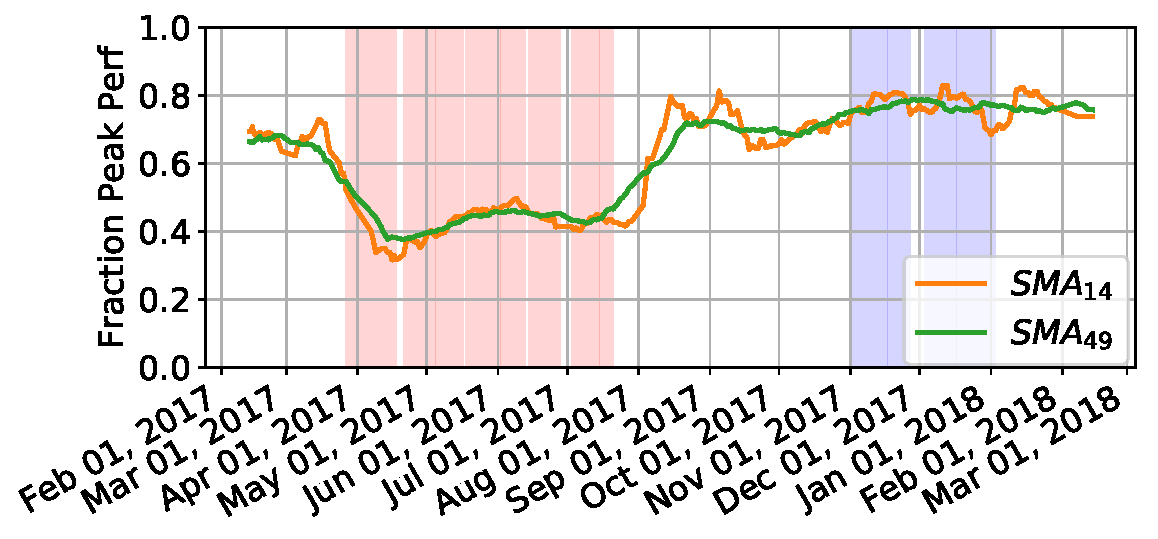
\includegraphics[width=1.0\columnwidth]{cscratch-bimodal-fsaveosscpu}
    \vspace{-.35in}
    \caption{Regions of negative correlation (red) and positive correlation (blue) between fraction peak performance and data server load during trend regions identified on \cori.
    SMAs for \cori's HACC write workload also shown to illustrate the coincidence of a long-term performance issue with the direction of correlation.}
    \label{fig:cscratch-bimodal-fsaveosscpu}
    % source: sc18_region-correlation-all.ipynb
\end{figure}


Another noteworthy feature that this method reveals is the bimodality of correlation between performance and the CPU load of the file system data servers (``Data Server Load'' in Fig. \ref{fig:trend-correlations}) on the Lustre-based test platforms.
A time-resolved view of the regions where performance correlates with data server CPU loads (Fig. \ref{fig:cscratch-bimodal-fsaveosscpu}) reveals that the bimodality of the correlation matches the biomodality observed in the HACC write workload on the affected storage systems.
During the long-term performance regression discussed in Section \ref{sec:features/timedependent}, high CPU load on the Lustre OSSs coincided with low performance of the I/O performance probes.
As soon as performance was restored on August 10, the relationship reversed, and high CPU load was observed favorably with respect to performance.

The positive correlation between performance and CPU load is consistent with the data servers using CPUs primarily to service incoming I/O requests, whereas the negative correlation indicates that another CPU load (as may be caused by an algorithmic bug) was present and competed with the data servers' ability to use CPU to service those same requests.
From this, we conclude that not only does baseline I/O performance vary with time, but \textbf{the nature and magnitude of how different attributes correlate with I/O performance also change over time}.
Had this correlation analysis been performed without partitioning over divergence regions, the regions of positive and negative correlation would have obfuscated each other in the net result.

The remaining two attributes that were found to correlate with performance
are file system fullness and \texttt{open(2)} coverage factor (a
measure of metadata resource contention).  The two instances of file
system fullness correlating negatively with performance are clear
and can be corroborated with independent observations from facilities
staff.  These two regions encapsulate periods when their respective
file systems approached 90\% fullness for a period of several days.
The observed loss of performance is consistent with Lustre's known
susceptibility to significant performance degradation as OSTs approach
90\% fullness~\cite{oral2014best,Lockwood2017}.

The correlation with
\texttt{open(2)} coverage factor is intuitive because this metric acts as a
proxy for metadata contention.  
One of these divergence regions was found to overlap with an unusually extensive, long-running multi-day purge of the \edison \scratchtwo file system.
However, it is unclear at this time what caused the other correlated divergence region.
% The above statement is not very satisfying, but we don't have time to do more detailed analysis.  The regions are:
% coverage_factor_opens 2017-03-29 19:11:51 - 2017-04-15 19:13:37 (71 points)
% coverage_factor_opens 2017-11-26 18:26:41 - 2017-12-13 20:03:11 (141 points)


\subsection{Transient performance loss} \label{sec:results/shortterm}

\begin{figure}

    \centering
    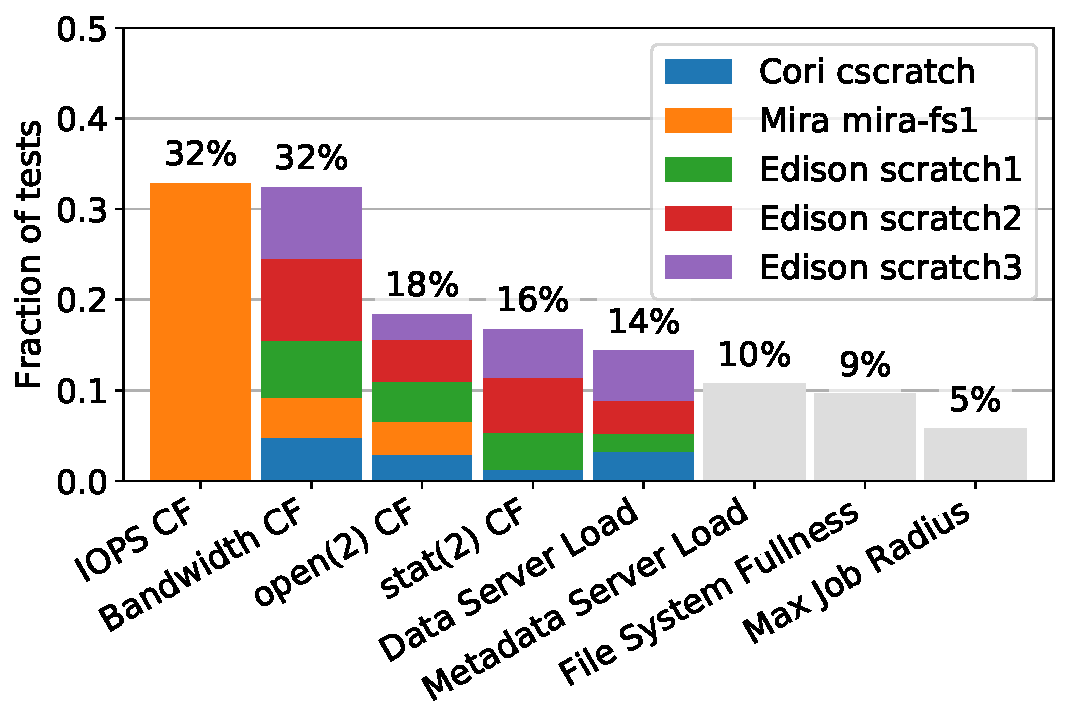
\includegraphics[width=1.0\columnwidth]{contributors-bad-by-system-grey}
    \vspace{-.35in}
    \caption{Attributes that correlated with poor I/O performance across all file systems and benchmarks tested normalized to the number of probes during which each attribute was measured.
    \mira was the only system for which IOPS coverage factor was measured.
    Greyed bars are attributes whose rate of classification were not statistically significant.
    Percentages do not add up to 100\% because multiple attributes are often classified as contributors for a single anomalous observation.
    }
    \label{fig:contributors-bad-by-system}
    % source: sc18_umamify-all.ipynb
\end{figure}

In addition to characterizing long-term performance issues, it is also advantageous to determine the reasons why I/O performance is severely degraded for one and only one day in an otherwise unremarkable period of time.
Such performance losses, exemplified as isolated dark blocks in Fig. \ref{fig:regions-heatmap}, may only be observed in one of the I/O performance probes issued on that day, suggesting a very short-lived issue that disappeared over the course of one or two of the eight daily probes.
The lack of a consistent performance trend surrounding these transients makes them difficult to correlate with other metrics as was done in the previous section, necessitating a different approach to characterizing them.

To address this need, we apply the same strategy of partitioning performance observations into divergence regions and then performing statistical analysis within each region.
To identify individual performance anomalies in a divergence region and classify the factors which contributed to them, we apply the following binary classification method:

\begin{enumerate}[leftmargin=*]

\item We examine the feature vector for every observation in the divergence region, and for each attribute $a$, determine the observation where that attribute's measured value was at its lowest, $\min(a)$.

\item We then define the \emph{anomalous observation} for the divergence region as the observation whose feature vector contains $\min(a)$ for fraction peak performance.
As divergence regions contain observations of similar performance by definition, this anomalous observation is truly anomalous-- it is differentiated from the long-term performance trends described in Sec.~\ref{sec:features} as well as the ones within its own divergence region.

\item Finally, we determine which other $\min(a)$ values also fall in this anomalous observation's feature vector and classify those attributes as contributors to the anomalous observation's performance.

\end{enumerate}

Qualitatively, this process codifies the conjecture that if I/O performance is anomalous on a specific day, the other measured attributes which were also anomalous at that time are what contributed to that behavior.
Quantitatively, this simple classification scheme allows us to identify relationships and define the statistical significance of each classification for individual anomalous observations using p-values\footnote{
The p-value is the probability of making a positive classification in the absence of an underlying relationship or, equivalently, the probability of positively classifying a random value.
Since there is only one $\min(a)$ in each region of $N$ observations, the p-value for our classifications is thus $\frac{1}{N}.$}.

The result of this process is zero or more attributes being positively classified as contributors to anomalous performance.
For example, if the lowest values of the bandwidth coverage factor and IOPS coverage factor attributes occur in the same feature vector as the lowest value for performance, we classify both bandwidth and IOPS coverage factors as contributors to that anomalous observation's performance.

To apply this method, we first group observations into sets of data by the test platform on which they ran as was done in Section \ref{sec:results/correlate-mira}.
These sets are then further subdivided according to I/O motif and read/write mode of the probe to classify anomalies at full temporal resolution and motif-level granularity.
The net result are $5 \times 4 \times 2 = 40$ sets of data, each representing a unique combination of test platform ($5 \times$, as listed in Table \ref{tab:platform-descriptions}), I/O motif ($4 \times$, per Table \ref{tab:benchmark-motifs}), and whether the probe was reading or writing ($2 \times$).
Schematically, each horizontal row in Figure \ref{fig:summary-heatmap} represents a single set.
For each set of observations, SMAs are calculated, crossover points are defined, and the set is partitioned into a set of divergence regions.

This partitioning results in 1,146 divergence regions across 40 sets of observations.
For each such region, we then apply the aforementioned binary classification to classify attributes that affected performance.
All statistically insignificant classifications ($\textup{p-value} > 0.10$) are discarded to eliminate divergence regions that are too small to make any meaningful classifications, and the final products are 
490 anomalous observations, of which 410 have at least one attribute positively classified.

As described in Section \ref{sec:methods/tokio}, not every observation's feature vector has every feature defined.
So as not to bias our results away from those attributes that were only measured for a subset of observations, we express the importance of each attribute as the number anomalous observations in which it was positively classified to the number of anomalous observations where it was measured.
Figure \ref{fig:contributors-bad-by-system} enumerates the attributes that were positively classified the most times.

As with the longer-term performance divergence characterized in Section \ref{sec:results/correlate-all}, high contention for bandwidth is found to also coincide with short-term performance transients.
However, contention for IOPS is also positively classified in a significant fraction of anomalous observations despite it not arising as a factor in longer-term performance divergence.
This contrast demonstrates that IOPS contention only becomes a statistically significant attribute related to performance degradation in short-term transients, and there are no sustained periods of high IOPS on \mirafsone.
This also distinguishes this utility of this transient classification from
the longer-term correlative analysis.
% Intuitively this result makes sense, as a job running on the machine performing I/O only places load on the metadata server during short duration events (eg. file open/close), whereas the load when the data is being read or written is likely to occur over much longer time periods.
% Intuitively, this result makes sense; a job performing I/O nominally places load on the metadata server only at the start and end of of reading and writing, while the process of reading and writing occurs over much longer time periods.
% \TODO{gkl: Phil/Shane, please review above line with your I/O expert hat on}

We also observe the coincidence of anomalous jobs and anomalous metadata coverage factor and CPU load on
data servers to a less significant degree.  This is
consistent with the moderate correlations shown in
Figure~\ref{fig:trend-correlations}.
Unlike the correlative analysis, however, metadata contention was found to impact individual jobs on every test platform and occurred at much higher frequency.
These findings indicate that metadata contention is much more likely to coincide with transient performance loss than a long-term and sustained divergence of performance.

In general, the contrast in correlations between transient events and
long-term trends shows that \textbf{the attributes that correlate with transient
performance problems (IOPS and
  metadata contention) often differ from those that correlate with
    long-term performance problems (bandwidth contention).} These are two distinct forms of performance variation that
require unique investigation techniques.

Metadata server CPU load, file system fullness, and maximum job radius were also classified in some anomalous observations.
However, the low number of anomalous observations in which they appeared calls into question the statistical significance of these three findings.
To address this, we calculate the p-values (the probability of observing the same number of classifications in the absence of a true underlying relationship) for each metric using binomial tests.\footnote{
We use one-tailed binomial tests with the number of positive classifications ($k$) and total observations ($n$) for each metric.
The fact that our dataset was filtered to only include regions with ${\textup{p-value} < 0.10}$ allows us to use 0.10 as a conservative value for the probability of success ($p$).}

These significance tests reveal that the number of times metadata server load, file system fullness, and maximum job radius were classified is statistically insignificant.
Whereas the leftmost five attributes in Fig. \ref{fig:contributors-bad-by-system} all have p-values of ${5 \times 10^{-5}}$ or lower, the insignificant metrics' are 0.15 or higher.
Qualitatively, these negative findings are not unreasonable; for example, file system fullness is most often a degenerative, long-term health problem as was identified in Section \ref{sec:results/correlate-all} and prior work~\cite{oral2014best,Lockwood2017}.
Thus, while it may coincide with transient anomalies, it is unlikely to be the sole contributor to poor performance on a single day.

The classification process and analysis described here demonstrates that it is possible to apply statistical analysis to fine-grained divergence regions and still obtain statistically significant insight into the causes of transient performance degradation.
While we chose a very simple binary classification criteria based on $\min{a}$, this process could be applied using any classification methodology that identifies relationships between feature vectors in a divergence region and quantifies the associated statistical significance.


\endinput

% NJW - this sentence adds too much complexity to end the section with
% 
%%%For example, classifying attributes based on quartiles rather than minima would be feasible with more coarse-grained divergence regions to offset the decrease in significance inherent in the selection criteria.

\subsection {Discussion}
\label{sec:results/discussion}

\TODO{This is where interesting dribs and drabs are winding up.  Do we carve out a separate section about this stuff, or just drop it?}

Our choice of averaging $\textup{SMA}_{short}$ over ${-0.5w_{short} <= t < +0.5w_{short}}$ makes it insensitive to choice of $w_{short}$.
For the analysis in Section \ref{sec:features/timedependent} changing $\textup{SMA}_{short}$ from $\textup{w}_{14}$ to both $\textup{w}_{7}$ and $\textup{w}_{28}$ resulted in no change to the dates bounding the 139-day divergence region.
The principal effect of changing $\textup{w}_{short}$ is the number of short regions that arise from the higher-frequency oscillations of $\textup{SMA}_{short}$ around $\textup{SMA}_{long}$.

\TODO{This is where a discussion about performance models having to account for long-term changes to baseline performance should go.  That doesn't seem to fit well into the rest of the narrative though.}

We found the exact choice of $w_{short}$ and $w_{long}$ to be somewhat arbitrary; adjusting these values by as much as $\pm 50\%$ did not affect the identification of the most significant events presented here.
In addition, a specific choice of $w$ does not preclude analyzing events longer or shorter than $w$, and we demonstrate methods to address this in Sections XYZ.

Although SMA crossover points are also applied in market analysis for detecting trends in prices and predicting when to buy or sell an asset based on the direction of the crossover~\cite{brock1992simple}.
However, the predictive value of SMA crossovers is a source of controversy even in the financial community, and thus, we focus here solely on using them as tools for detecting trends and partitioning divergent regions in historical datasets.

Financial market analysis techniques can be used to detect underlying trends within noisy I/O performance data.
